\documentclass[11pt]{report}
\usepackage[utf8]{inputenc}
\usepackage[english]{babel}
\usepackage{fancyhdr}
\usepackage[final]{pdfpages}
\setcounter{secnumdepth}{-1}
\usepackage{amsfonts}
\usepackage{float}
\pagestyle{fancy}
\usepackage{url}
\usepackage{graphicx}
\usepackage{fancyvrb}
\usepackage{alltt}
\usepackage{graphicx}
\usepackage{caption}
\usepackage{subcaption}
\usepackage{amsmath}
\usepackage{xr}
\usepackage{amssymb}
\usepackage{courier}
\nonstopmode
\pagestyle{fancy}
\lhead{Nikolaj Friis Østergaard - ltm741}
\rhead{\today}
\newcommand{\then}{\rightarrow}
\DeclareMathOperator*{\Bigcdot}{\scalerel*{\cdot}{\bigodot}}
\begin{document}
\section{1 Histogram-based processing}
\subsection{1.1}
TODO
\subsection{1.2}
If the image is normalized to have values in the range [0,1], then the PDF of a constant image is just the normalized histogram. The CDF is just
$$
y(x_k) = \sum_{j=0}^{k}p_x(x_k)
$$
The k'th entry is the sum of all previous entries.
For a constant PDF the CDF will just be a monotonically increasing, each step incremented by the same constant value.
\subsection{1.3}


\subsection{1.4}
\subsection{1.5}
Generally no, given an image transformed by a CDF, we have no way of knowing which intensities matched to which acummulated intensities.

\subsection{1.6}





\section{2 Image filtering and enhancement}

\subsection{2.1}
The approximation for the x value uses the difference between the pixel before and the pixel after. The y value is calculated the same way. This result in the kernel:
$$
K =
\begin{bmatrix}
  -1 & 0 & 1
 \end{bmatrix}
$$

The imfilter function can either use correlation or convolution, the default is correlation. Correlation and convolution are almost the same, but convolution flips the kernel, on both axis. So the resulting kernel for the simle approximation approach is with convolution is
$$
K =
\begin{bmatrix}
  1 & 0 & -1
 \end{bmatrix}
$$
For kernels like gaussian, which are symetrical around the center, it does not matter which we choose to use, since kernels that will run over the image for the correlation and convolution will be the same.
\subsection{2.2}

The kernel in 4.5.2.1 shows the kernel for the x derivative, and thus these will be used for discussion. Instead of just looking at the pixel to the right and the left, we also use the information about the row above and below. By using the row above and below, we don't interpret a single noise pixel as being part of and edge, since the pixels below and above does not indicate that there is a continiued edge. This makes noise get lower values then real edge, which spanned multiple rows. The same logic is applied for the y derivative, where we look at the derivatives and both sides. Sobel weigh the current rows pixels heigher the the ones below and above. Were Prewitt weigh them equally.

\subsection{2.3}
Figure \ref{fig:2_3_0} shows the eight.tif image with both salt and pepper noise and gaussian noise, filtered with mean and median filter. The first column shows the image with salt and pepper noise with a mean filter, the second column is the image with gaussian noise filtered with mean filter. The third column shows the iamge with salt and pepper noise, filtered with a median filter and the fourth column shows the image with gaussian noise, with a median filter. The first row has a windows size of 3, the second window size of 5 and the third a window size of 7. Looking at the first column we can see how increasing windows size improves the denoising, but also the edge blur a bit. In the second column we see again how increasing the windows size improves the denoising. For the median filter the salt and peper in column 3 is as good as gone in the first image, with windows size 3, increasing the window size only blurs the image a bit more, and makes the background brighter. In column 4 with gaussian noise we see that the increase in window size improves the denoising, while bluring the image, about as much as with the mean filter.

\begin{figure}[!ht]
    \centering
    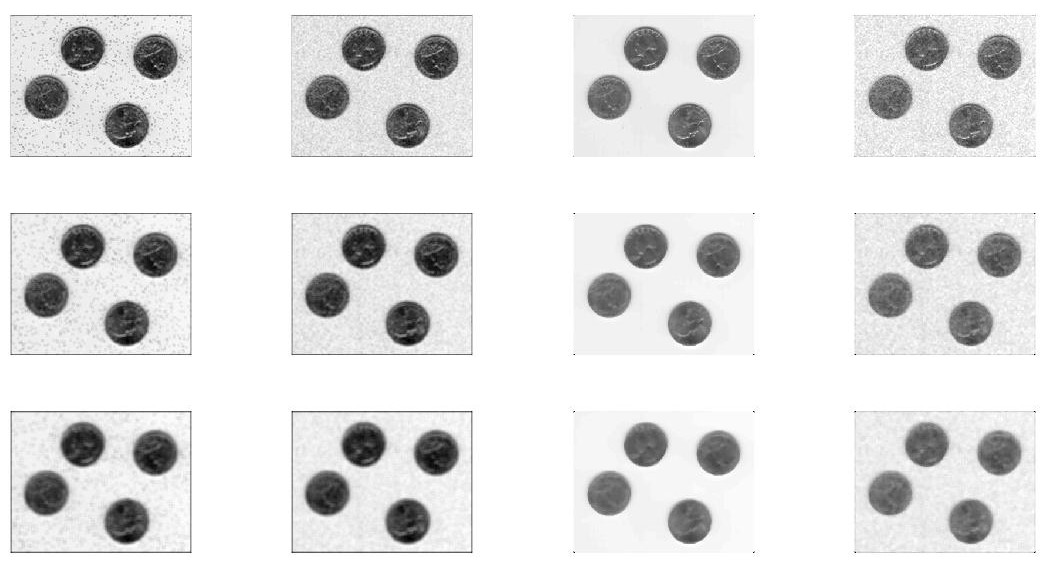
\includegraphics[width=1\textwidth]{fig23_0.jpg}
    \caption{mean and median filter on salt/peper noise and on gaussian noise for different window sizes}
    \label{fig:2_3_0}
\end{figure}

Figure \ref{fig:2_3} shows the computaional cost for increasing window sizes. Th blue line is median filter, red is mean filter. As we can see, median filter is generally more expensive to use, compared to the mean filter. Another thing to notice is that the median filter has a lower computational cost when the windows size is odd. It also looks like the median filter spikes more, and increases in computaional cost, when N becomes bigger, see when $N \geq 21$ on the graph, compared to the mean filter, which seems to be increasing at a steady pace.

\begin{figure}[!ht]
    \centering
    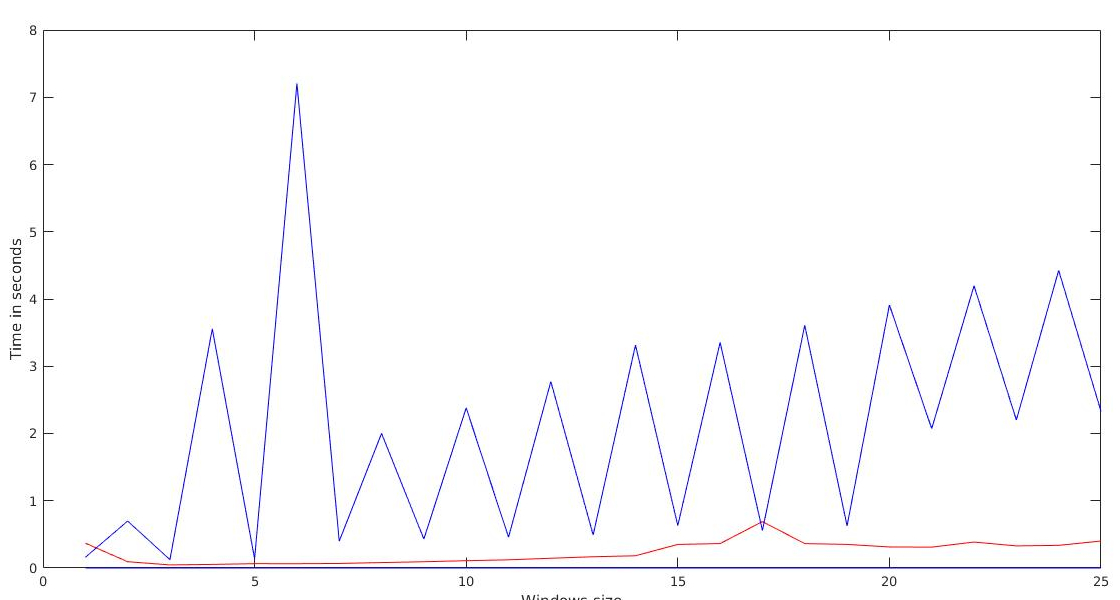
\includegraphics[width=1\textwidth]{fig23.jpg}
    \caption{The computational cost of doing mean filter and median filter, based on window size.}
    \label{fig:2_3}
\end{figure}

\subsection{2.4}
Figure \ref{fig:2_4} shows the eight.tif, with salt and pepper noise, filtered with a gaussian kernel where $\sigma = 5$, with windows size in the range 3:19, with increments og 2, to keep the kernel diameter odd. We can see how the difference between image 5 and image 8, are less notacible then the difference between image 2 and image 5. This is because with a smaller windows, the image is blurred less. At some point the windows is so big, that the values furthest away from the center are so small, that their weight is neglectable, thus increasing the windows size show no notacible difference. And that is why its easier to see the difference between image 2 and 5 then image 5 and 8.

\begin{figure}[!ht]
    \centering
    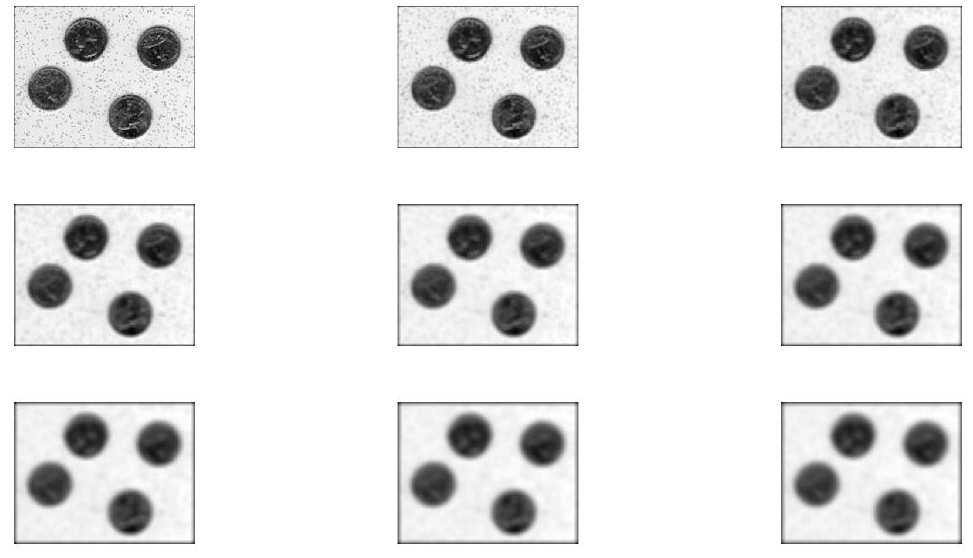
\includegraphics[width=1\textwidth]{fig24.jpg}
    \caption{9 Images with inceasing windows size starting at 3 ending at 19.}
    \label{fig:2_4}
\end{figure}



\subsection{2.5}

Figure \ref{fig:2_5} show the eight.tif, with salt and peper noise, filtered with a gaussian filter, with increasing $\sigma$ starting at 1 and ending at 17, in incremental steps of 2. The windows size N is 3*sigma + 1, and then rounding up to nearest odd integer. What we can see that increasing $\sigma$ and windows size, rapidly improves the noise reduction, but also blures the edges to an equal extend. In image 4, the noise is as good as gone, so from there on, the only difference is just that the edges in the following images are more blurred out. So increasing the $\sigma$ and windows size does makes the filter more effective at removing noise, but also makes finding edges harder. The noise removal is not something that improves the larger $\sigma$, since when sigma = 7 and window size = 23, the noise is gone, and we can't do better then remove it.
\begin{figure}[!ht]
    \centering
    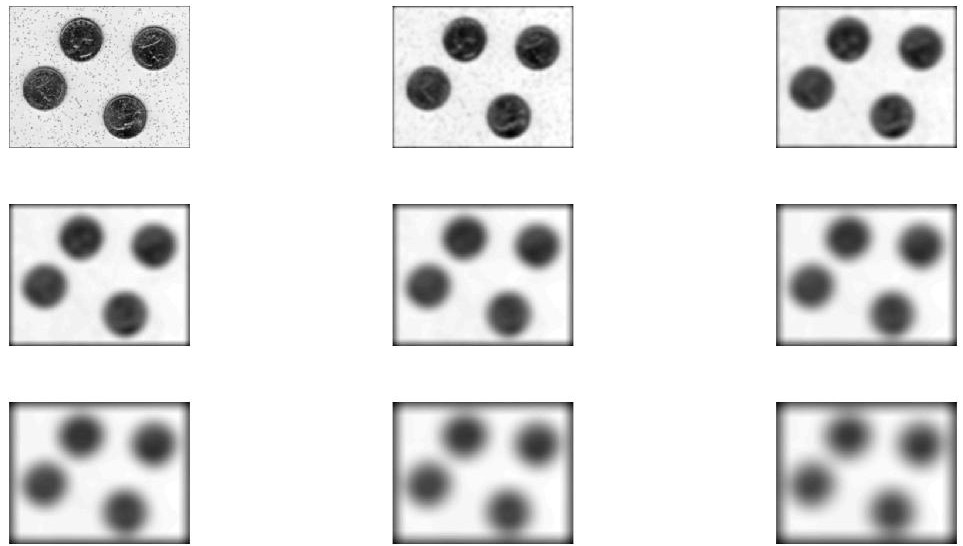
\includegraphics[width=1\textwidth]{fig25.jpg}
    \caption{9 Images with inceasing sigma and windows size starting at sigma = 1 and ending at sigma = 17, with increments of 2.}
    \label{fig:2_5}
\end{figure}

\section{3 Bonus question}


\end{document}
